\chapter{Эксперимент РЭД-100} 
\label{chapt2}
В 2021-22 гг. на реакторе четвертого энергоблока Калининской АЭС был поставлен эксперимент РЭД-100 по исследованию УКРН ~\cite{The_RED100_Experiment}. Это один из немногих экспериментов, поставленных на промышленном реакторе. РЭД-100 был создан прицельно для измерения УКРН. Постановке эксперимента на Калининской АЭС предшествовал длительный подготовительный процесс в ЛЭЯФ НИЯУ МИФИ, включавший в себя наладку оборудования и инженерные запуски. 
\section{Детектор РЭД-100}
\label{sect2_1}
\subsection{Устройство детектора РЭД-100}
\label{subsect2_1_1}
Детектор РЭД-100 представляет собой двухфазный эмиссионный детектор. Рабочим веществом данного детектора является ксенон, однако данный детектор может быть модифицирован для работы и с другими благородными газами. Схема детектора РЭД-100 приведена на рисунке \ref{img:detscheme}. Общий вес ксенона в системе РЭД-100 составляет около 200 кг, при этом вес непосредственно рабочего объема, участвующего в регистрации частиц -- 130 кг. 
\begin{figure}[H]	\center{\includegraphics[width=0.5\linewidth]{images/red100.png}}
	\caption[Принцип работы и устройство детектора РЭД-100] {[Принцип работы и устройство детектора РЭД-100. 1 --- внешний сосуд титанового криостата, 2 --- внутренний сосуд титанового криостата, 3 --- верхняя матрица из девятнадцати ФЭУ типа Hamamatsu R11410-20, 4 --- сетчатый анод и электронный затвор, 5 --- рабочий объем, окруженный тефлоновым отражателем со встроенными полезадающими электродами, 6 --- сетчатый катод, 7 --- нижняя матрица из девятнадцати ФЭУ, 8 --- нижний центральный теплосъемник с термосифоном, 9 --- медная обойма для нижней матрицы ФЭУ, 10 --- медный кожух холодного сосуда криостата, 11 --- один из двух боковых теплосъемников с термосифонами, 12 --- медная обойма верхней матрицы ФЭУ, 13 --- гибкий тепловой мост, 14 --- верхний центральный теплосъемник с медным диском, на котором конденсируется ксенон, 15 --- теплоизолирующий подвес, 16 --- сильфонная тепловая развязка для вывода кабелей; $e^-$ --- электроны ионизации, $\overline{\nu}$ --- антинейтрино, передающее энергию ядру отдачи, S1 --- сцинтилляционная вспышка, S2 --- электролюминесцентная вспышка.}
	\label{img:detscheme}
\end{figure}

\par Внутренний объем криостата (2) содержит электродную структуру, необходимую для создания электрических полей в детекторе. Основная электродная структура состоит из сетчатых электродов катода (6), расположенного снизу, гейта и анода (4) для создания однородного сильного электрического поля в газовой фазе над поверхностью жидкости, а также системы полезадающих колец. Сетчатые электроды представляют из себя плоские травленые сетки из нержавеющей стали с гексагональными ячейками, обладающие коэффициентом оптической прозрачности около 80\%. Они обеспечивают небольшое дрейфовое поле в жидкости; поле, вытягивающее электроны из жидкости в газ, а также сильное поле в газе, в котором происходит электролюминесценция. Система полезадающих колец состоит из 20 кольцевых (12-гранных) эквидистантных электродов, создающих равномерно распределенный электрический потенциал по высоте дрейфового объема. 
\par Рабочий объем детектора заключён внутри электродной системы и просматривается фотоэлектронными умножителями (ФЭУ) Hamamatsu R11410-20, размещенными в виде двух матриц – верхней (3) и нижней (7), по 19 ФЭУ в каждой. Этот тип ФЭУ специально разработан японской фирмой Hamamatsu для низкофоновых эмиссионных детекторов на жидком ксеноне. Фотоумножители предназначены для работы при криогенных температурах (-100°С) и чувствительны к длине волны 175 нм с эффективностью регистрации квантовой эффективностью порядка 30\%. Каждый из установленных в детекторе ФЭУ прошел предварительную процедуру характеризации при комнатной температуре, включающую измерение одно-фотоэлектронных характеристик, темнового счета, временных спектров следования после-импульсов и ряда других параметров\cite{Akimov2017}. Характеризация ФЭУ показала, что они имеют хорошее одно-фотоэлектронное разрешение и достаточно высокое внутреннее усиление ($\sim 5\cdot10^6$) сигнала при средних величинах напряжения питания $\sim 1500$ В. 
\par Рабочий объем представляет собой 12-гранную призму с боковыми гранями, выполненными из светоотражающих тефлоновых пластин. Пространство между полезадающими кольцами и стенками внутреннего корпуса криостата заполнено тефлоном, играющим роль вытеснителя ксенона. Фотоумножители располагаются в специальных медных обоймах (9) и (12), которые находятся в тепловом контакте с верхним (14) и нижним (8) термосифонными теплосъёмноками. Тепловой контакт с верхним теплосъёмником осуществляется при помощи гибкого теплового моста, изготовленного из многослойной медной фольги (13). Боковая поверхность внутреннего сосуда криостата снаружи покрыта медным кожухом для выравнивания температурных градиентов. На медном кожухе установлены боковые термосифонные теплосъемники (11).
\par
\begin{figure}[ht]
  \begin{minipage}[ht]{0.64\linewidth}    \center{\includegraphics[width=1.0\linewidth]{images/red100grids.pdf} \\ а)}
  \end{minipage}
  \hfill
  \begin{minipage}[ht]{0.34\linewidth}  \center{\includegraphics[width=1.0\linewidth]{images/red100electrodes.pdf} \\ б)}
  \end{minipage}
  \caption[Схема и фото электродной системы детектора РЭД-100] {Схема (а) и фото (б) электродной системы детектора РЭД-100. А – сетчатый анод; С – сетчатый катод; В и Т – экранирующие сетчатые электроды под земляным потенциалом; G1 и G2 – сетчатые электроды электронного затвора; Field shaping rings – медные полезадающие электроды;  Resistor chain – цепочка резисторов между полезадающими электродами для создания между ними разности потенциалов. Все размеры приведены в мм.}
  \label{img:red100electrodes}  
\end{figure}

\begin{figure}[ht]	\center{\includegraphics[width=0.9\linewidth]{images/PMT_map_21.06.2017 (1).pdf}}
	\caption[Расположение фотоумножителей в матрице считывания.] {Cлева – в верхней, справа – в нижней; в обоих случаях показан вид сверху; значком -HV показана ориентация матриц относительно катодного высоковольтного кабеля; LED – положения светодиодов вблизи верхней матрицы}
	\label{img:pmtscheme}
\end{figure}

\par Детальное устройство детектирующей части, состоящей из электродной структуры и двух матриц фотоэлектронных умножителей, показано на рисунке \ref{img:red100electrodes} (а). Схема расположения ФЭУ показана на рисунке \ref{img:pmtscheme}. Электродная система включает T - экранирующий электрод верхней матрицы фотоумножителей, находящийся постоянно под земляным потенциалом; А – анод, на который подается положительный потенциал порядка +5 кВ; G2 – подповерхностный электрод, обеспечивающий сильное электрическое поле в газовой фазе детектора, на который подается потенциал порядка -5 кВ; G1 – электрод, обеспечивающий блокировку прохождения электронов к поверхности в случае, когда в детекторе произошло событие с очень большим энерговыделением (описание работы затвора см. ниже), потенциал на нем в режиме пропускания электронов поддерживается равным потенциалу электрода G1, в режиме блокировки потенциал смещается на +300 В; С – катод, потенциал которого -12 кВ; B – экранирующий электрод нижней матрицы, находящийся постоянно под земляным потенциалом. Для создания равномерного электрического поля в дрейфовой области в тефлоне между электродами G1 и C размещены круговые полезадающие электроды. Потенциал на этих электродах задается равномерным делителем собранным между электродами G1 и C при помощи резисторов с сопротивлением 1 ГОм (рисунок \ref{img:red100electrodes} (б)). Полное сопротивление делителя 18 ГОм.
\par Все сетки в детекторе электрополированные и изготовлены из фольги из нержавеющей стали толщиной 0.2 мм с электролитически сформированными гексагональными открытыми ячейками (оптический коэффициент прозрачности ~0.8). Внутренний размер шестиугольного отверстия ячейки - 3.5 мм, ширина перемычки между соседними ячейками 0.2 мм. Сетки в натянутом состоянии приварены точечной контактной сваркой к кольцам из нержавеющей стали.
\parТакже в РЭД-100 были реализованы технологии электронного затвора и блокировки ФЭУ с целью недопущения непреднамеренной регистрации больших сигналов от космических мюонов. 

	
Событие, соответствующее прохождению космического мюона через детектор, представляет собой практически непрерывное свечение, образованное выходом большого количества электронов с трека мюона в газовую фазу. Поскольку мюон  в среднем теряет в объеме детектора около 200 МэВ, сигнал электролюминесценции оказывается слишком большим для нормальной работы фотоумножителей, что при длительном воздействии такой сильной засветки на фотокатоды приводит к их деградации. Для предотвращения “выгорания” фотокатодов фотоумножителей производится выключение эмиссии фотоэлектронов с фотокатодов путем подачи на 1-ые диноды (одновременно всех фотоумножителей) положительного смещения величиной около 300 В (равной характерной разности потенциалов между фотокатодом и первым динодом). Этот сигнал вырабатывается триггерным модулем по приходу сцинтилляционного сигнала, превышающего соответствующий амплитудный порог. Данный сигнал также подается на электронный затвор (на электрод G2) для предотвращения прохождения электронов от мюона в область электролюминесценции. Предотвращение прохождения электронов к поверхности жидкого ксенона при большом энерговыделении в рабочем объеме позволяет снизить шум одиночных электронов за счет минимизации компоненты, вызванной спонтанным выходом с поверхности электронов, находящихся там в потенциальной яме. Более подробно данные технологии, а также устройство детектора РЭД-100 описано в диссертации А. В. Хромова \cite{Khromov_thesis}.

\subsection{Система циркуляции и очистки}
\label{subsect2_1_2}
%+более общие слова, что мы меряем ионизационный сигнал и нам не нужно его терять
\parОсновным источником измеряемого сигнала в детекторе РЭД-100 является электролюминесценция, производимая электронами ионизации. При дрейфе электронов к границе раздела фаз происходят потери, связанные с захватом дрейфующих электронов электроотрицательными примесями. Для минимизации этих потерь требуется тщательная подготовка рабочего вещества. В процессе хранения и транспортировки чистота рабочего вещества деградирует и требуется дополнительная циркуляция через очищающие геттеры, так как детекторы, подобные РЭД-100 требуют особо высокой чистоты рабочего вещества. Для измерения чистоты ксенона мы опираемся на производное выражение в виде среднего времени жизни свободных электронов в жидком ксеноне. 
%спросить у акимова, что со связью концентрации и времени жизни
%TODO подумать про то как модифицировать текст этого абзаца
\parСистема газообеспечения (система хранения и очистки газа и система вакуумной откачки) установки РЭД-100 включает в себя стандартные газовые элементы, такие как баллоны высокого давления для хранения ксенона, безмасляные вакуумные насосы, элементы газовых коммуникаций, циркуляционный насос, манометры и вакуумметры с металлическими уплотнениями, электронные элементы контроля давления газа и вакуума, горячий металлический геттер SAES MonoTorr. Система позволяет осуществлять циркуляционную очистку ксенона по замкнутому контуру и поддерживать необходимый уровень чистоты ксенона. Газовая система детектора РЭД-100 является системой закрытого типа, то есть не имеющей контакта с атмосферой. При неработающем детекторе РЭД-100 ксенон хранится в алюминиевых баллонах Luxfer под давлением 50 атмосфер. 
\parДетектор соединён с газовой системой через интерфейсный блок при помощи трех сильфонных металлорукавов внутренним диаметром 68 мм и длиной 4 м. Один из этих металлорукавов содержит высоковольтные кабеля, другой - сигнальные кабеля, третий - сильфонный теплообменник для минимизации теплопритока при циркуляции ксенона через систему очистки ксенона. При работе детектора металлорукава продуваются постоянным потоком газообразного ксенона, поступающего из системы очистки с потоком порядка 1 л/мин. На входе в газовую систему каждый канал циркуляции оборудован контрольным расходомером MKS1479D.  Поток газа в каждой линии устанавливается и регулируется программным образом. После прохождения газообразного ксенона через геттер газообразный ксенон возвращается в детектор по замкнутому контуру, конденсируется и в жидком виде поступает в детектор. 

\subsection{Система термостабилизации}
\parДля охлаждения детектора RED-100 и поддержания его при температуре жидкого ксенона используется криогенная система, основанная на термосифонной технологии (гравитационная тепловая труба)~\cite{red100cryo}. Эта технология имеет ряд преимуществ по сравнению с другими известными системами охлаждения и термостабилизации: уменьшенное количество радиоактивных элементов вблизи активного объема детектора, значительно более низкий уровень механических колебаний, низкий расход хладагента и способность работать без электроэнергии. Термосифон криогенной системы RED-100 представляет собой вертикально ориентированную закрытую трубку, которая может быть функционально разделена на следующие три части: сверху - конденсатор, погруженный в сосуд Дьюара со свободно кипящим жидким азотом; внизу испаритель (охлаждающая головка), термически контактирующий с детектором, и пассивная адиабатическая часть между этими двумя частями. Трубка заполнена газообразным азотом. Эффективный отвод тепла от детектора достигается фазовым переходом азота внутри термосифона. Газ конденсируется в конденсаторе и стекает в испаритель. Там он закипает от тепла, отводимого от детектора, и поднимается вверх к конденсатору, и таким образом, процесс непрерывно циклически повторяется. Теплопроводность термосифонов может достигать очень высоких значений, порядка нескольких десятков кВт/К·м, что сопоставимо с теплопроводностью углеродных нанотрубок. Термостабилизация детектора RED-100 осуществляется путем изменения тепловой проводимости термосифона (охлаждающей способности), что, в свою очередь, осуществляется путем изменения количества газообразного азота внутри трубки, соединяющим теплосъёмник, установленным в месте поглощения тепловой энергии, с конденсором, установленным внутри термосифонного сосуда Дьюара, в котором происходит ожижение азота. В детекторе RED-100 имеются четыре термосифона с общей мощностью охлаждения до $\sim$ 400 Вт.
\parТермосифонная криогенная система обеспечивает конденсацию около 200 кг жидкого ксенона в течение порядка суток (до 10 л/мин газа при н.у., или 60 г/мин) и позволяет поддерживать жидкий ксенон внутри детектора RED-100 при постоянной температуре в диапазоне от 165 до 175 К с точностью <0,2 К, а также обеспечивать вертикальный градиент температуры <1 К/м, чтобы минимизировать конвекционные потоки жидкого ксенона внутри чувствительного объема, которые могут повлиять на характеристики детектора.

\subsection{Система сбора данных}
\label{subsect2_1_3}
Сбор данных осуществляется с помощью специализированной системы и заключается в приеме сигналов из детектора, усилении/формировании этих сигналов, генерации триггера и сохранении оцифрованных данных на диск. Эти действия производятся модулями электроники и компьютером data acquisition (DAQ). Система является централизованной. 
\par В рамках эксперимента РЭД-100 требуются надежные идентификация и измерение одиночных фотоэлектронов ФЭУ в рамках окна записи больше максимального времени дрейфа в электролюминесцентном зазоре, поэтому производится запись полных форм сигналов. 
\parПосле регистрации фотонов ФЭУ формируют электрические сигналы, выведенные из детектора через интерфейсный модуль. Сигналы усиливаются быстрыми малошумящими усилителями Phillips Scientific 777. Усилители имеют полосу пропускания от 0 до 200 МГц и регулируемый коэффициент усиления в диапазоне 2x–50x, что обеспечивает дополнительную свободу для выравнивания усиления ФЭУ. Сигнал с усилителей отправляется непосредственно на АЦП, а также на линейный разветвитель Phillips Scientific 748 для формирования триггера. Для записи форм сигналов используются модули аналого-цифрового преобразования (АЦП) прямого преобразования CAEN V1730. Модули обеспечивают оцифровку форм сигналов с частотой 500 млн. отсчетов/с и разрешением 14 бит, память модуля позволяет хранить 5 млн. отсчетов для каждого канала. В режиме максимальной чувствительности модуль обеспечивает шаг бинирования 0.03 мВ и 2 нс, что вполне достаточно для надежной регистрации одиночных фотоэлектронов. В основном режиме работы детектора ФЭУ работают в режиме, обеспечивающем амплитуду одно-фотоэлектронных импульсов $\sim$ 1 мВ.

\textbf{Триггер}
\parБольшие различия основных режимов работы накладывают повышенные требования на схему формирования триггера, как в части нижнего порога, так в отношении динамического диапазона. Для решения всех возложенных задач триггерная схема реализована на базе цифрового модуля программируемой логики CAEN V1495. Общая схема триггера приведена на рисунке \ref{img:trigger}. Режим наибольшей чувствительности оптимизирован на отбор событий с сигналами от 1 до 10 электронов ионизации. Его работа построена на пересчёте количества срабатываний поканальных дискриминаторов (CAEN V895), настроенных на порог $\sim$1/3 от амплитуды однофотонных импульсов, в бегущем окне длиной 2 мкс, что соответствует длине электролюминесцентного сигнала. Подсчет ведется независимо по верхним и нижним плоскостям ФЭУ, срабатывание происходит если количество импульсов укладывается в выбранный диапазон, что позволяет отбрасывать случайные совпадения и большие сигналы.
\begin{figure}[H]
	\center{\includegraphics[width=1.0\linewidth]{images/trigger.png}}
	\caption{Блок-схема триггера}
	\label{img:trigger}
\end{figure}
\parДля отбора гамма-квантов производится суммарный сигнал по верхней и нижней плоскостям ФЭУ, получаемый с помощью линейных сумматоров CAEN N625. Эти сигналы отправляются на дополнительные АЦП, которые отправляют результат непосредственно в триггерный модуль. В модуле производится цифровая обработка формы сигналов, что позволяет отбирать события с совпадениями сцинтилляционных и электролюминесцентных сигналов в пределах времени полного дрейфа. Отбор мюонов осуществляется по совпадению сигналов с дискриминаторов с большим порогом (~1В) в нескольких ФЭУ. Триггерный модуль формирует сигналы на блокировку ФЭУ и затвора. Дополнительно триггерный модуль используется для мониторинга состояния детектора путём определения частоты различных событий.


\subsection{Методы калибровки детектора РЭД-100}
\label{subsect2_1_4}
РЭД-100 является крайне сложным и чувствительным прибором. Для детального понимания процессов внутри детектора требуется измерение следующих значений:
\begin{itemize}
    \item площади однофотоэлектронных импульсов SPE (single photo electron) для каждого канала
    \item параметры сигнала (светосбор, длительность) от одного электрона ионизации
    \item параметры эффективности светосбора в детекторе
    \item время жизни электронов при дрейфе в жидкой фазе
    \item ионизационный выход (количество электронов ионизации на единицу энерговыделения в рабочей среде детектора)
    \item коэффициент экстракции электронов при переходе границы раздела фаз
\end{itemize}
\par Для определения указанных параметров необходима комплексная калибровка систем детектора. 
	\parК калибровочным данным можно отнести light emitting diod (LED) калибровку, данные с одноэлектронными (SE -- single electron) сигналами, мюонные данные и гамма калибровочные данные. С некоторыми отличиями, приведенные калибровочные типы данных набирались как при инженерных запусках детектора, так и при постановке эксперимента на Калининской АЭС.
 \begin{enumerate}
     \item\textbf{LED калибровка}
    \parПри наборе данного типа данных триггер запускался от генератора одновременно со светодиодом, расположенного как показано на рисунке \ref{img:pmtscheme}. Это позволяло набрать данные с SPE импульсами и определить параметры однофотоэлектронных импульсов для каждого ФЭУ.
	 \item\textbf{SE-данные}
	\par Цель набора данного типа калибровок -- получение информации о одноэлектронных сигналах с нулевым порогом регистрации. Был использован внешний триггер не зависящий от сигнала внутри детектора. Реализация данного триггера была различной при различных запусках детектора и описана в соответствующих разделах (\ref{subsect2_2_1}, \ref{subsect2_2_2}). Также этот метод позволяет измерить частоту сигналов SE-фона.
	 \item\textbf{Мюонные данные}
	\parНабор мюонных данных используется для определения времени жизни электронов при дрейфе в жидком ксеноне и контроля степени очистки, описанной в разделе \ref{subsect2_1_2}. Для набора данных от космических мюонов детектор переводился в специальный режим, характеризующийся отключением электронного затвора, а также пониженным (до 0.1 мВ на SPE) напряжением на ФЭУ. Отбор мюонов осуществляется по совпадению сигналов с дискриминаторов с большим порогом ($\sim$1В) в нескольких ФЭУ. 
	 \item\textbf{Измерения с гамма-источниками}
	\parБыли использованы гамма-источники $^{60}$Co, $^{22}$Na и $^{137}$Cs. Триггер в данном случае запускался от сцинтилляции. Измерения с гамма-источниками необходимы для энергетической калибровки отклика детектора, измерения энергетического разрешения, а также для построения так называемых функций эффективности светосбора (light response functions -- LRF). Более подробно про LRF и процедуры пространственного восстановления см. \ref{sect3_2}
\end{enumerate}

\subsection{Основные источники фона в детекторе}
\label{subsect2_1_5}
Как и любой детектор, РЭД-100 подвержен воздействию различного типа фонов. Источники фона в РЭД-100 можно разделить на две большие группы:
\begin{enumerate}
    \item Внешние источники фона. К внешним источникам фона относится гамма и нейтронный фон различной природы от окружающих материалов. Также фон от космических мюонов, которые дают гигантский ионизационный сигнал. 
    \item Внутренние источники фона. К внутренним источникам фона относятся, во-первых распады радиоактивных элементов в рабочем веществе детектора, а во-вторых, так называемый фон спонтанной эмиссии, зарегистрированный также и на других детекторах такого типа~\cite{se_akimov, Santos:2011ju}, включающий в себя несколько компонент. Первая компонента вызвана спонтанным выходом электронов с поверхности жидкости, находящихся там в потенциальной яме. Оставшаяся компонента шума представляет собой электроны, вышедшие с трека с задержкой, либо захваченные и с задержкой высвобожденные электроотрицательными примесями (в настоящее время природа данной компоненты остается до конца не выясненной). Наложение подобных задержанных сигналов от многих последовательно приходящих мюонных сигналов образует перманентный фон. Совпадение двух или больше таких сигналов по времени формирует неточечные события, составляющие существенную часть фона. Более подробно об алгоритмах подавления данных событий см. \ref{sect4_2}.
\end{enumerate}

\subsection{Программный пакет REDOffline}
\label{subsect2_1_6}
Для первичной обработки форм сигналов с различных детекторов в ЛЭЯФ НИЯУ МИФИ был разработан программный пакет REDOffline. Несмотря на скрупулезный подход к сбору электроники детектора, на сырых формах сигнала имеются электрические наводки, не всегда известной природы. В программном пакете REDOffline реализована полиномиальная коррекция наводок. 

Следующим этапом обработки, необходимым для всех данных в виде форм сигналов является поиск нулевой линии. Для данной процедуры создается амплитудная гистограмма для каждого канала, среднее значение на которой принимается за нулевую линию.

Завершающий этап первичной обработки -- распознавание и параметризация импульсов на форме сигналов. В REDOffline поиск импульсов реализован с использованием амплитудного порога, зависящего от стандартного отклонения шумовой дорожки.

\parКак правило, перед любыми процедурами анализа данные детектора РЭД-100 проходили обработку пакетом REDOffline, что существенно ускоряло и упрощало дальнейшую работу с данными.


\section{Конфигурация установки при различных наборах данных}
\label{sect2_2}
\subsection{Инженерный запуск в ЛЭЯФ НИЯУ МИФИ 2019 г.}
\label{subsect2_2_1}
\begin{figure}[H]
	\center{\includegraphics[width=0.8\linewidth]{images/red100_2019setup.png}}
	\caption[Схема установки при инженерном запуске в МИФИ.] {1 -- сосуд Дьюара с жидким азотом, 2 -- криостат термосифонной криогенной системы, 3 -- пассивная защита, 4 -- детектор РЭД-100, 5 -- интерфейсный модуль, 6 -- система очистки ксенона, 7-8 -- хранилище для ксенона, 9 -- система управления термосифонами, 10 -- система сбора данных}
	\label{img:2019scheme}
\end{figure}
В 2019 с помощью детектора был проведен инженерный сеанс установки РЭД-100. Основными целями данного теста являлись проверка различных систем установки, измерения фона и калибровка детектора гамма-источниками. Более подробная информация про данный сеанс и его результаты находится в статье \cite{RED100_2019}. %Конфигурация установки представлена на рисунке \ref{img:2019scheme}. 
\par В рамках данного теста набирались калибровочные данные:
 \begin{enumerate}
     \item LED-калибровка
     \item Мюонные данные
     \item SE-данные. Набор данных производился следующим образом: сохранялись 300 мкс, предшествовавшие срабатыванию триггера на гамма-кванты.
     \item Гамма-калибровки. Для калибровки использовались источники $^{60}$Co и $^{22}$Na. Источник $^{60}$Co был сколлимирован, а при наборе данных с $^{22}$Na была задействована схема совпадений с детектором NaI. 
 \end{enumerate}

\subsection{Эксперимент на Калининской АЭС 2021-22 гг.}
\label{subsect2_2_2}
Калининская АЭС расположена недалеко от города Удомля Тверской области. Состоит из четырех энергоблоков общей мощностью 4000~МВт. 
\begin{figure}[H]
	\center{\includegraphics[width=1.0\linewidth]{images/kaes_red100_scheme.jpg}}
	\caption[Схема установки на Калининской АЭС] {Схема установки на Калининской АЭС. 1 -- бак термосифонной системы, 2 -- поддерживающая бак конструкция, 3 -- водный бак, 4 -- медная защита}
	\label{img:kaesscheme}
\end{figure}

\begin{figure}[H]
  \begin{minipage}[ht]{0.49\linewidth}
    \center{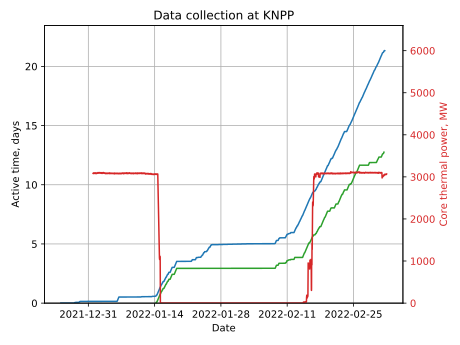
\includegraphics[width=1.0\linewidth]{images/cumulative-time-power.pdf} \\ а)}
  \end{minipage}
  \hfill
  \begin{minipage}[ht]{0.49\linewidth}
    \center{\includegraphics[width=1.0\linewidth]{images/type-pie.pdf} \\ б)}
  \end{minipage}
	\caption[Соотношение набранных типов данных и мощности реактора]{Соотношение набранных типов данных и мощности реактора. Слева -- график мощности реактора (красная линия) и объем набираемых данных различных типов (синяя линия -- все данные, зеленая -- УКРН-подобные данные), справа -- круговая диаграмма показывающая соотношение количества набранных данных различных типов}
	\label{img:datadiagram}
\end{figure}
Детектор РЭД-100 располагался в 19 метрах снизу от реактора 4 энергоблока. В в качестве основной пассивной защиты от космических мюонов выступали бетонные перекрытия здания энергоблока. Далее конструкция детектора была помещена в мягкий бак из ПВХ диаметром 5 м, наполненный водой, что обеспечивало пассивную защиту от нейтронов толщиной 60 см. Для защиты от гамма фона вокруг детектора была выстроена конструкция из медных брусков толщиной 5 см. Схема пассивной защиты детектора РЭД-100 приведена на рисунке \ref{img:kaesscheme}. Более подробная информация о пассивной защите детектора РЭД-100 находится в статье \cite{shielding}.
Мощность реактора в процессе набора данных менялась, ее график приведен на рисунке \ref{img:datadiagram}.  Данные набирались в периоды как с включенным, так и с выключенным реактором для сравнения спектров. 
	Всего набирались шесть основных типов данных:
 \begin{enumerate}
     \item LED-калибровки
     \item Мюонные данные
     \item SE-данные
     \item Гамма-фон
     \item Гамма-калибровки
     \item УКРН-подобные данные
 \end{enumerate}
Соотношение объемов набранных данных различных типов приведено на круговой диаграмме на рисунке \ref{img:datadiagram}.
\parПомимо измерений основным детектором РЭД-100, непрерывно проводились измерения с использованием вспомогательных детекторов, которые были необходимы для понимания фоновых условий эксперимента. К вспомогательным детекторам относятся сцинтилляционные детекторы NaI[Tl] и Bicron, а также два датчика уровня радона Radex.
\parНа протяжении набора данных проводились измерения внешнего гамма-фона, которые показали что фон однороден за исключением нескольких отдельных областей~\cite{The_RED100_Experiment}. Измеренный гамма-фон в помещении на КАЭС приблизительно в 5 раз больше, чем в ЛЭЯФ НИЯУ МИФИ. Это связано с толстыми бетонными стенами, потолком и полом в здании реактора.  На протяжении сеанса набора данных на КАЭС вспомогательный детектор NaI[Tl] был расположен как показано на рисунке \ref{img:kaesscheme}. На рисунке \ref{img:gammaneutronbckg} (а) показан график изменения гамма-фона на протяжении сеанса набора данных. Резкие изменения в начале и в конце набора данных связаны с заполенением бака водной защиты и его осушением, соответственно.
\par Результаты мониторинга нейтронного фона при постановке эксперимента на КАЭС показаны на рисунке \ref{img:gammaneutronbckg} (б). Заметной разницы между нейтронным фоном при включенном и при выключенном реакторе не наблюдалось. 
\par Фон от космических мюонов измерялся непосредственно детектором РЭД-100, так как мюонные данные были необходимы для измерения времени жизни электронов в жидком ксеноне. Мюонный фон также был стабилен во время постановки эксперимента. 

\begin{figure}[H]
  \begin{minipage}[ht]{0.49\linewidth}
    \center{\includegraphics[width=1.0\linewidth]{images/NaI_count_rate_monitoring.png} \\ а)}
  \end{minipage}
  \hfill
  \begin{minipage}[ht]{0.49\linewidth}
    \center{\includegraphics[width=1.0\linewidth]{images/neutrons_rate.png} \\ б)}
  \end{minipage}
  \caption[Графики изменения гамма и нейтронного фонов.]{а) График изменения гамма-фона (измерения суммировались за каждые 3 часа набора данных). б) График изменения нейтронного фона}
  \label{img:gammaneutronbckg}  
\end{figure}

\section{Моделирование отклика детектора РЭД-100}
\label{sect2_3}
Для понимания отклика детектора на различные взаимодействия необходимо детальное моделирование. На данный момент не существует программных пакетов, позволяющих моделировать полную цепь происходящих в детекторе процессов, поэтому было произведено последовательное моделирование в трех различных пакетах. Кроме того, был написан собственный модуль для моделирования временных разверток сигналов.
\subsection{Модель РЭД-100 в различных программных пакетах}
\label{subsect2_3_1}
\textbf{Модель РЭД-100 в GEANT4}
\parРезультат описывающегося теоретическими моделями взаимодействия ионизирующих частиц с веществом моделируется в GEANT4 при помощи методов Монте-Карло~\cite{ALLISON2016186}. GEANT4 — широко используемый в экспериментальной физике программный пакет. GEANT4 предоставляет возможность создания моделей детекторов, состоящих
из различных материалов и использующих различные электрические поля и симулирует поведение частиц в различных частях детектора (например, предоставляя возможность оценить процент отсечения фона защитой). Так же GEANT4 позволяет отслеживать не только конечные частицы, но и промежуточные процессы и их параметры.
\par GEANT4-модель детектора РЭД-100 представляет собой практически полную модель реального детектора. В данном программном пакете происходит моделирование только первичных взаимодействий частицы с рабочим веществом, которое происходит в жидкой фазе. Последующий дрейф электронов в жидкости и газе, а также оптические процессы моделируются с использованием других инструментов.

\par\textbf{Модель РЭД-100 в NEST}
%\label{subsect2_3_2}
\parОсновная функция GEANT — моделирование процессов взаимодействия частиц с материалами, энергопотерь и т.д. Отдельная задача — понимание и моделирование сцинтилляции, ионизации и электролюминесценции. Модуль GEANT-scintillation хоть и позволяет приблизительно оценить численные характеристики данных процессов, но для детального моделирования требуется большая проработанность теоретических моделей и экспериментальных данных. Эту нишу в области моделирования процессов в детекторах на жидких благородных газах занимает NEST. NEST представляет собой программный модуль для предсказания процессов энерговыделения в жидких благородных газах, основанный на совмещении полуэмпирических моделей и экспериментальных данных с разных экспериментов. Более подробно про NEST изложено в кандидатской диссертации Е. Козловой \cite{Kate_thesis}. 
Характеристики детектора РЭД-100, полученные с использованием модели РЭД-100 в NEST:
\begin{enumerate}
    \item Отношение ионизации к сцинтилляции
    \item Количество фотонов электролюминесценции от одного электрона ионизации
    \item Скорость дрейфа электронов в жидкости
\end{enumerate}

\par\textbf{Модель РЭД-100 в ANTS2}
%\label{subsect2_3_3}

ANTS-2 — программный пакет, разработанный для моделирования оптических процессов и обработки данных позиционно-чувствительных детекторов \cite{Morozov_2016}. Также ANTS-2 позволяет задавать оптические свойства материалов и границ между ними, после чего моделировать распространение фотонов от сцинтилляции и электролюминесценции. Плюсом данного пакета является возможность проследить путь каждого фотона от момента возникновения до попадания на фотокатод ФЭУ. 
Кроме того, в данном программном пакете реализованы алгоритмы пространственного восстановления с использованием light response functions (LRFs).
\parВ данном программном пакете была создана детальная оптическая модель детектора РЭД-100, включающая титановый криостат, тефлоновый отражатель, электроды-сетки и кольца-держатели. Данная оптическая модель позволяет проследить путь каждого фотона от рождения до поглощения материалами или регистрацией ФЭУ. 
\subsection{Модель временных разверток}
\label{subsect2_3_2}
Для изучения сигналов в несколько электронов ионизации требуется моделирование временных разверток сигналов электролюминесценции, которые представляют собой раскладку по времени и каналам регистрации для всех зарегистрированных фотонов. 
\parЭлектроны ионизации после возникновения дрейфуют к границе раздела фаз, при это подвергаясь диффузии как по оси Z, так и в плоскости XY. Диффузия описывается следующим образом \cite{EXO-200:2016qyl}:
\begin{equation}
n(\vec{x}, t)=\frac{N}{4 \pi D_T t \sqrt{4 \pi D_L t}} \exp \left[\frac{-\left(x^2+y^2\right)}{4 D_T t}\right] \times \exp \left[\frac{-\left(z-v_d t\right)^2}{4 D_L t}\right]
\label{diffusion}
\end{equation}
\par Параметр $D_L$ в данном случае был принят равным $25 см^2$/c \cite{Njoya:2019ldm}.
Диффузия в плоскости XY не учитывалась, так при прохождении через электроды-сетки электроны концентрируются в центрах ячеек, размер которых сильно превышает масштаб диффузии на рассматриваемой глубине.
\par Сигнал от одиночного электрона ионизации моделируется следующим образом:
\begin{enumerate}
    \item Для точек, расположенных в центрах ячеек электрода-сетки рассчитывается относительная вероятность для каждого ФЭУ зарегистрировать фотон, испущенный из этой точки. В данном случае используется приближение о том, что все фотоны электролюминесценции испускаются из одной точки. 
    \item Для каждого фотона в соответствии с равномерным разыгрывается координата испускания внутри электролюминесцентного зазора.
    \item Количество фотонов разыгрывается в соответствии с распределением Гаусса, парметры которого подбираются таким образом чтобы (в конце концов все сошлось) среднее значение которого рассчитывается исходя из экспериментального распределения суммарного светосбора в центре детектора и отношения суммарной относительной вероятности в конкретной точке к соответствуеющему значению в центре детектора. (с учетом положения). Среднеквадратичное отклонение складывается из Пуассоновского размытия и дополнительной компоненты неизвестной природы.
    \item Истинная длительность события (непосредственно время дрейфа электрона через электролюминесцентный зазор) разыгрывается в соответствии с распределением Гаусса с параметрами, подобранными экспериментально. 
    \item Исходя из истинной длительности события, координаты испускания фотонов, полученные на шаге 2, пересчитываются во времена испускания. Так как скорость света на данных масштабах расстояний можно считать достаточно большой, времена испускания соответствуют временам регистрации фотонов.
\end{enumerate}

Для создания сигналов от нескольких электронов ионизации требуется скомбинировать несколько событий от одного электрона ионизации. При этом время начала электролюминесценции для каждого SE размывается в соответствии с формулой \ref{diffusion} и скоростью дрейфа в жидкости, рассчитанной при помощи пакета NEST. Реализация описанной в данном разделе симуляции написана автором на языке python 3.8. Пример визуализации смоделированного описанным выше способом события представлен на рисунке~\ref{img:simulationevent}

\begin{figure}[H]
  \center{\includegraphics[width=0.6\linewidth]{images/simulation_event_example.pdf}}
  \caption[Пример смоделированного с использованием LRF из оптической модели события в 3 SE.] {Пример смоделированного с использованием LRF из оптической модели события в 3 SE. Различными цветами (значками) обозначены фотоны, возникшие от разных электронов ионизации.}
  \label{img:simulationevent}  
\end{figure}